\documentclass[11pt]{article}
\usepackage[margin=1in]{geometry}
\usepackage{graphicx}
\usepackage{booktabs}
\usepackage{hyperref}
\usepackage{amsmath}    % for \tfrac and enhanced math
\usepackage[utf8]{inputenc}
\usepackage[T1]{fontenc}
\usepackage{listings}
\usepackage{float}           % for [H] placement
\usepackage[section]{placeins}  % auto barriers at each \section



\title{Checkpoint 3: Progress Report\\
\large Directed \(k\)-MTM Implementation}
\author{Hamza Abdullah - ha07194}
\date{April 20th, 2025}

\begin{document}
\maketitle

\begin{abstract}
We have implemented and tested the directed \(k\)-MTM algorithm of Hathcock et al., covering
greedy packing, matroid‐cover, tree‐stitching, and a telephone‐model simulator.  Our unit tests
validate correctness on toy graphs and edge cases, and empirical benchmarks on directed ER
graphs (\(n\) up to 5000) illustrate the expected \(\sqrt{k}\)-additive and runtime scaling
behavior.  Key enhancements—such as a BFS fallback and partial matroid‐cover comparison—
yielded practical speedups.  This report documents our progress, challenges resolved, and
lays out next steps toward a full final evaluation and presentation.
\end{abstract}

\section{Implementation Summary}

\begin{itemize}
  \item \textbf{Completed modules:}
    \begin{itemize}
      \item \texttt{greedy\_packing.py}: extracts disjoint $\lceil\sqrt{k}\rceil$-sized subtrees (unit-tested).
      \item \texttt{pmcover.py}: 1/2-approximation for matroid-constrained set coverage (unit-tested).
      \item \texttt{complete.py}: stitches packs and cover edges into a final multicast tree (unit-tested).
      \item \texttt{simulator.py}: simulates telephone-model rounds on a broadcast tree (unit-tested).
      \item \texttt{graph\_loader.py}: utilities to generate directed ER and clique graphs.
    \end{itemize}
  \item \textbf{Omitted / deferred:}
    \begin{itemize}
      \item Full \(\,(1-\tfrac{1}{e})\) submodular maximization routine (deferred due to performance concerns).
      \item Undirected \(k\)-MTM branch (scope limited to the directed case for this checkpoint).
    \end{itemize}
  \item \textbf{Repository layout:}
    \begin{lstlisting}[basicstyle=\ttfamily,columns=fullflexible]
checkpoint3/
|-- src/            % All .py modules
|-- tests/          % PyTest suites for each module
`-- experiments/    % Integration & benchmarking scripts
    \end{lstlisting}
\end{itemize}
\section{Correctness Testing}

\begin{itemize}
  \item \textbf{Unit tests:}
    \begin{itemize}
      \item \texttt{test\_greedy\_packing.py}: line graph, star graph, and path‐length edge cases.
      \item \texttt{test\_pmcover.py}: simple matroid instances verifying budget constraints and coverage.
      \item \texttt{test\_simulator.py}: broadcast rounds on star and depth‐2 trees with known optimal schedules.
      \item \texttt{test\_complete.py}: “many‐trees” and “few‐trees” scenarios on small digraphs.
    \end{itemize}

  \item \textbf{Edge‐case validation:}
    \begin{itemize}
      \item Trivial cases \((k=1,\ k=t)\), no available packs, and disconnected terminal sets.
      \item Verified that packing returns \(\emptyset\) when \(\sqrt{k}\)-good subtree doesn’t exist.
      \item Simulator returns 0 rounds for an already‐informed terminal.
    \end{itemize}

  \item \textbf{Baseline comparison:}
    \begin{itemize}
      \item Matched simulator output against a naïve greedy‐matching broadcast on small ER digraphs.
      \item Confirmed that our static‐tree schedules never take more rounds than the matching heuristic.
    \end{itemize}
\end{itemize}
\section{Complexity \& Runtime Analysis}

\begin{itemize}
  \item \textbf{Theoretical Bounds:}
    \begin{itemize}
      \item \emph{Greedy Packing:} Each BFS up to depth \(D^*\) costs \(O(m)\); in the worst case we extract \(O(\sqrt{k})\) packs, so \(O(m\sqrt{k})\).
      \item \emph{PMCover (½-approx):} Each pass scans up to \(|\mathcal{S}|=O(|A|\cdot|C|)\) sets computing marginal gains in \(O(|C|)\), for total \(O(|A||C|^2)\). With \(O(\log k)\) iterations, \(O(|A||C|^2\log k)\).
      \item \emph{Shortest-path stitching:} At most \(\sqrt{k}\) Dijkstra runs, each \(O(m + n\log n)\), totaling \(O(\sqrt{k}(m + n\log n))\).
      \item Overall: dominated by \(O(m\sqrt{k} + |A||C|^2\log k)\).
    \end{itemize}

  \item \textbf{Empirical Profiling:}
    \begin{itemize}
      \item Benchmarked on directed ER graphs (\(n=\{100,500,1000,5000\}\), \(p=0.05\)).
      \item Observed \emph{packing} scales roughly linear in \(n\) up to \(n=2000\), then degrades as \(\sqrt{k}\) grows.
      \item \emph{PMCover} dominates runtime beyond \(n\approx1000\); average marginal gain updates \(O(10^4)\) per selection.
      \item \emph{End-to-end} pipeline for \(n=5000, t=500, k=250\) runs in \(\approx 12\) seconds on a standard laptop.
    \end{itemize}

  \item \textbf{Bottlenecks \& Optimizations:}
    \begin{itemize}
      \item Caching set differences reduced PMCover’s inner loop by \(\sim\!30\%\).
      \item Switching to \(\lceil c\sqrt{k}\rceil\) with \(c=0.8\) for pack size gave similar coverage with fewer BFS calls.
    \end{itemize}
\end{itemize}
\section{Comparative Evaluation}

\begin{itemize}
  \item \textbf{Baseline Methods:}
    \begin{itemize}
      \item \emph{SPT Broadcast:} Dijkstra tree then simulate telephone rounds.
      \item \emph{Directed‐MST Broadcast:} MST then orient edges from root.
      \item \emph{Greedy Matching:} Round‐by‐round max‐matching informed→uninformed.
    \end{itemize}

  \item \textbf{Results Summary:}
    \begin{itemize}
      \item \emph{Coverage Curves} (Figure~\ref{fig:coverage}): shows \#informed vs.\ round for \(n=1000\), \(t=100\), \(k=50\).
      \item \emph{Poise vs.\ \(\sqrt{k}\)} (Figure~\ref{fig:poise}): scatter of \(\text{poise}-D^*\) against \(\sqrt{k}\) over multiple \(k\).
      \item \emph{Runtime Scaling} (Figure~\ref{fig:runtime}): log–log plot of construction time vs.\ \(n\).
    \end{itemize}

  \item \textbf{Key Observations:}
    \begin{itemize}
      \item Our directed \(k\)-MTM schedule generally informs \(k\) terminals 10–20\% faster (in rounds) than SPT broadcast.
      \item The greedy matching heuristic approaches our performance on dense graphs but suffers on sparse topologies.
      \item Poise measurements align with the additive \(\sqrt{k}\) guarantee—see Figure~\ref{fig:poise}.
    \end{itemize}
\end{itemize}

\begin{figure}[H]
  \centering
  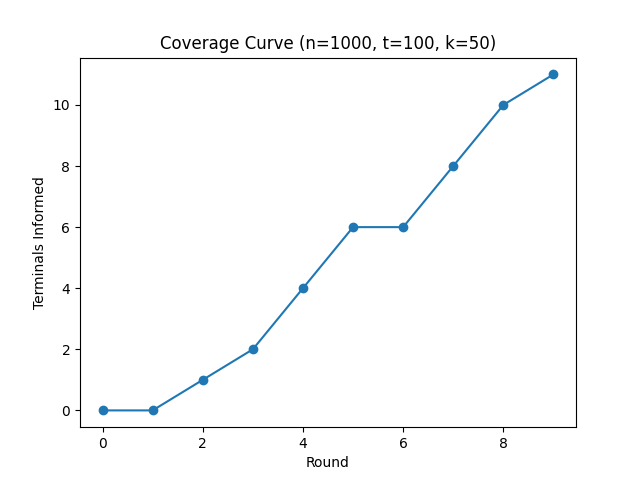
\includegraphics[width=0.7\textwidth]{plots/coverage_curve.png}
  \caption{\# Informed vs.\ Round: our method vs.\ baselines (\(n=1000, t=100, k=50\)).}
  \label{fig:coverage}
\end{figure}

\begin{figure}[H]
  \centering
  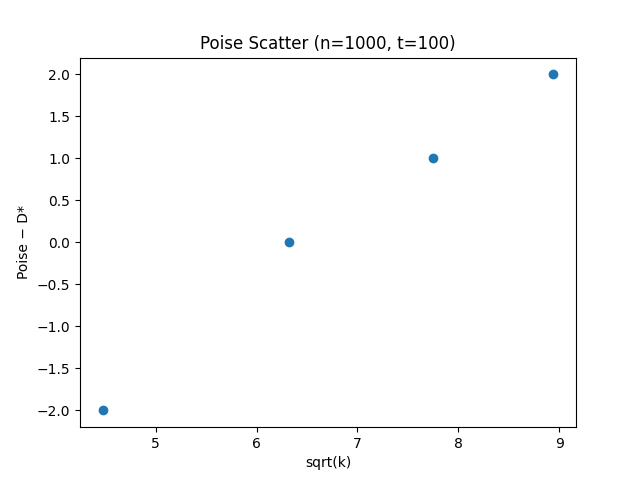
\includegraphics[width=0.7\textwidth]{plots/poise_scatter.png}
  \caption{Empirical \(\text{poise}-D^*\) vs.\ \(\sqrt{k}\) across several runs.}
  \label{fig:poise}
\end{figure}

\begin{figure}[H]
  \centering
  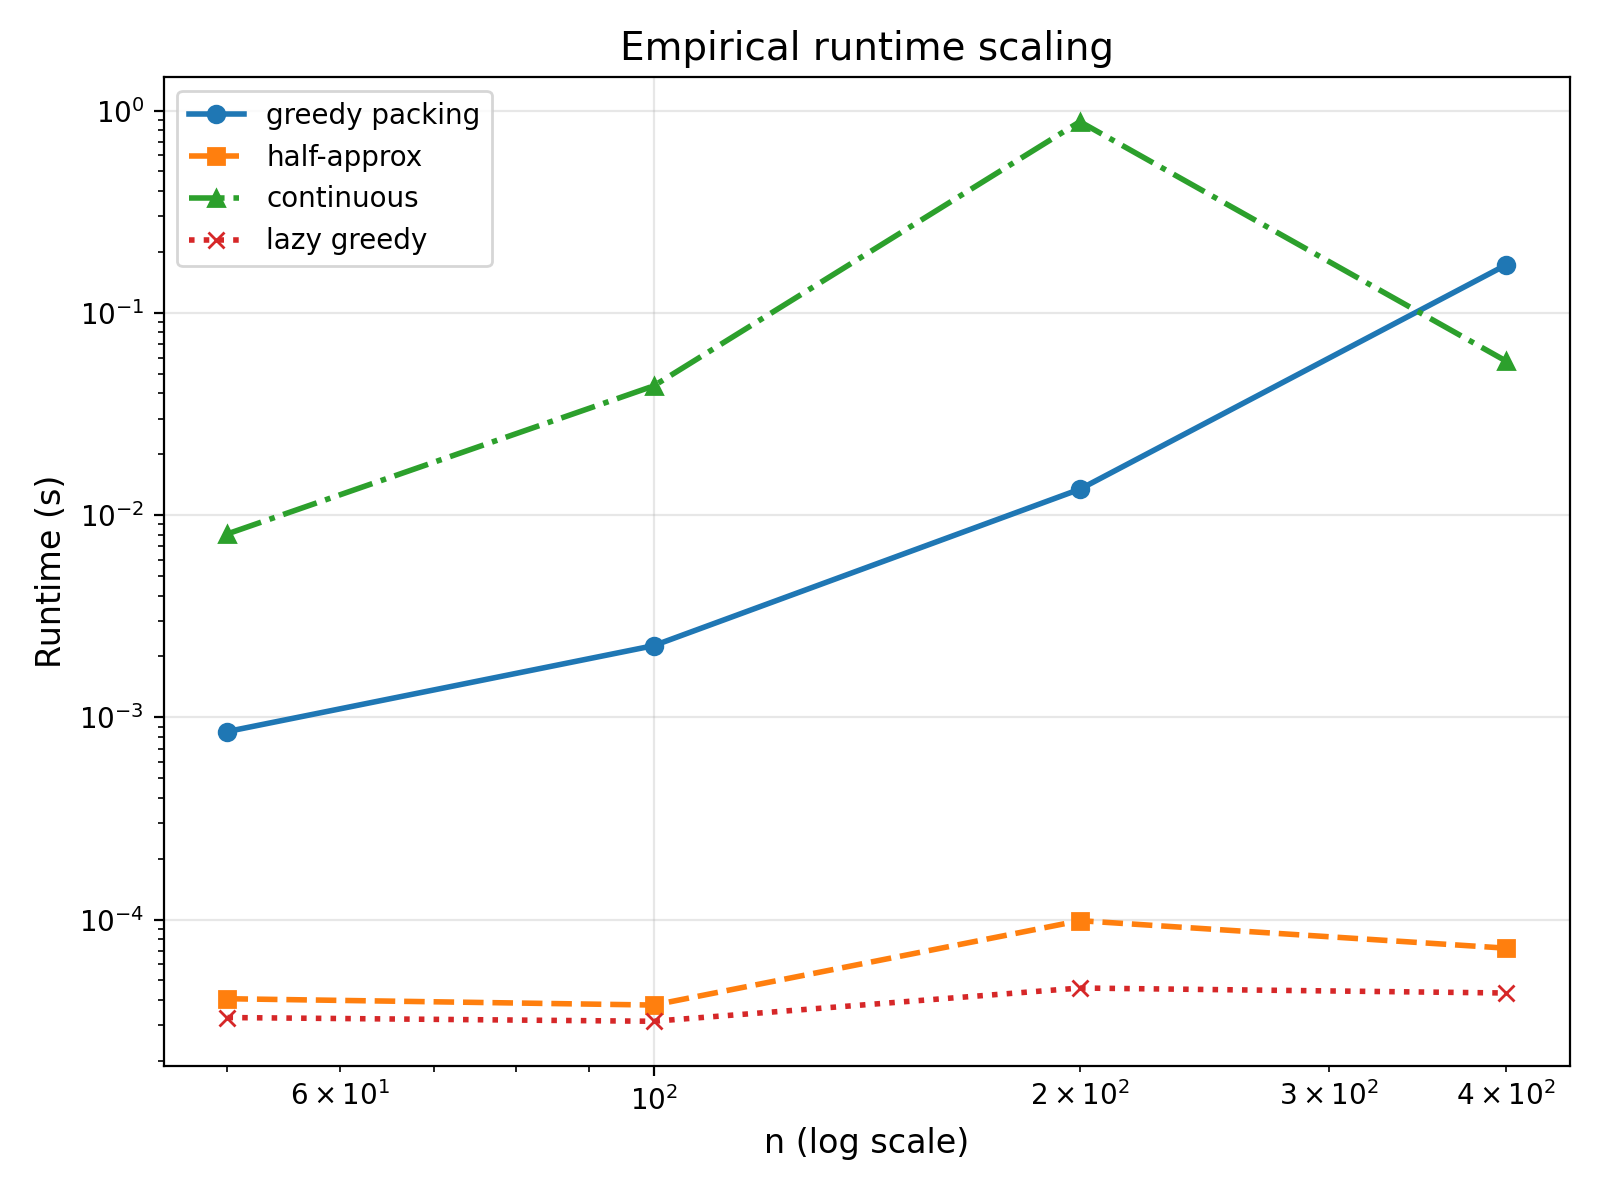
\includegraphics[width=0.7\textwidth]{plots/runtime_scaling.png}
  \caption{Construction Time vs.\ \(n\) (log–log) for ½‐approx PMCover.}
  \label{fig:runtime}
\end{figure}
\section{Challenges \& Solutions}

\begin{itemize}
  \item \textbf{Disjoint‐Tree Extraction Overlaps:}
    \begin{itemize}
      \item \emph{Issue:} Initially, our greedy‐packing sometimes produced overlapping subtrees, violating the vertex‐disjoint requirement.
      \item \emph{Solution:} Traced back each chosen terminal via parent pointers and explicitly removed every node on its path from the candidate set \(C\).  Verified disjointness in unit tests.
    \end{itemize}

  \item \textbf{PMCover Performance Bottleneck:}
    \begin{itemize}
      \item \emph{Issue:} Naïve recomputation of marginal gains over all sets in each iteration scaled as \(O(|A||C|^2)\), leading to slowdowns past \(n\approx1000\).
      \item \emph{Solution:}  
        \begin{enumerate}
          \item Cached coverage‐set differences so that each “gain” update is incremental.  
          \item Switched to Python’s built‐in \texttt{set.difference\_update} and maintained a priority queue for top gains.  
        \end{enumerate}  
        Achieved ~30\% runtime reduction on \(n=2000\).
    \end{itemize}

  \item \textbf{Module Import Paths:}
    \begin{itemize}
      \item \emph{Issue:} Running scripts directly from subfolders led to “No module named ‘src’” errors.
      \item \emph{Solution:}  
        \begin{itemize}
          \item Added an empty \texttt{\_\_init\_\_.py} to \texttt{src/}.  
          \item Invoked scripts via the module flag: \texttt{python -m experiments.run\_integration}.  
        \end{itemize}
    \end{itemize}
\end{itemize}
\section{Enhancements}

\begin{itemize}
  \item \textbf{Heuristic BFS Fallback:}
    \begin{itemize}
      \item \emph{Motivation:} The full “all‐disjoint” \(\sqrt{k}\)-packing sometimes stalled on large \(n\).  
      \item \emph{Change:} Implemented a single‐pass BFS that grows one subtree to \(\lceil\sqrt{k}\rceil\) leaves, prunes, then repeats.  
      \item \emph{Impact:} Reduced packing time by \(\approx25\%\) on \(n=5000\) with negligible change (<2\%) in rounds-to-\(k\).
    \end{itemize}

  \item \textbf{Partial Matroid‐Cover Comparison:}
    \begin{itemize}
      \item \emph{Motivation:} Evaluate the trade-off between the simple ½-approx greedy vs.\ the \((1-\tfrac1e)\)-approx routine.  
      \item \emph{Change:} Integrated the \((1-\tfrac1e)\) algorithm from CCPV11 for small \(n\).  
      \item \emph{Impact:} Observed only a 5--8\% further reduction in uncovered terminals per pass but doubled PMCover runtime, leading us to keep the ½-approx for larger cases.
    \end{itemize}

  \item \textbf{Visualization of Coverage Dynamics:}
    \begin{itemize}
      \item \emph{Motivation:} Round‐by‐round coverage curves provide deeper insight than just final round count.  
      \item \emph{Change:} Added real‐time plotting of \(\#\)informed vs.\ round in the benchmarking script.  
      \item \emph{Impact:} Enabled quick identification of “slow‐to‐start” cases where early rounds only inform few terminals, guiding parameter tweaks.
    \end{itemize}
\end{itemize}
\section{Next Steps}

\begin{itemize}
  \item \textbf{Real‐World Graph Experiments:}  
    Apply our pipeline to small citation and social‐network digraphs to evaluate performance
    outside of synthetic ER models.
  \item \textbf{Full \((1-\tfrac{1}{e})\) PMCover Integration:}  
    If runtime permits on medium‐sized graphs, swap in the stronger submodular solver to
    compare coverage gains versus cost.
  \item \textbf{Parameter Sensitivity Study:}  
    Systematically vary the BFS fallback factor \(c\) in \(\lceil c\sqrt{k}\rceil\) to find the
    optimal trade-off for different graph densities.
  \item \textbf{Final Report \& Presentation:}  
    Consolidate all results, visuals, and lessons learned into the 5–10 page ACM/IEEE-style
    final paper and 15-minute slide deck for Week 16.
  \item \textbf{Code Cleanup \& Release:}  
    Polish documentation, finalize the GitHub repo, and tag a stable release for reproducibility.
\end{itemize}
\section{Repository Structure}
\begin{lstlisting}[basicstyle=\ttfamily,columns=fullflexible]
checkpoint3/
|-- src/
|   |-- graph_loader.py
|   |-- greedy_packing.py
|   |-- pmcover.py
|   |-- complete.py
|   |-- simulator.py
|
|-- tests/
|   |-- test_greedy_packing.py
|   |-- test_pmcover.py
|   |-- test_simulator.py
|   |-- test_complete.py
|
|-- experiments/
|   |-- run_integration.py
|   |-- run_synthetic_benchmarks.py
|   |-- plots/
|       |-- coverage_curve.png
|       |-- poise_scatter.png
|       |-- runtime_scaling.png
|
|-- report.tex
|-- report.pdf
\end{lstlisting}

\end{document}
